%==============================================================================
\section{Application: Hypothetical Thrombolytic MRCT Using GUSTO-I Data}\label{sec:application}
%==============================================================================

We illustrate the nABCD framework through a hypothetical scenario grounded in publicly available data from GUSTO-I, a large international trial in acute myocardial infarction (AMI). A sponsor is developing a novel thrombolytic agent (Drug~T) for AMI and is planning a Phase~3 MRCT across multiple regions. At the planning stage, the sponsor uses publicly available individual patient data (IPD) from GUSTO-I ($N = 40{,}830$; 16 anonymized regions)\cite{gusto1993} to assess distributional similarity of candidate effect modifiers across regions and to identify suitable pooling partners for a designated anchor region.

\subsection{Scenario Design and Effect Modifier Selection}\label{sec:app_scenario}

The FTT Collaborative Group\cite{ftt1994} meta-analysis of fibrinolytic therapy trials established age as a confirmed effect modifier for thrombolytic efficacy in AMI: the absolute mortality reduction varied from approximately 1\%pt in patients aged $<55$ to 3.4\%pt in those aged 55--74, declining to non-significant in patients aged $\geq75$. From these published subgroup-specific treatment effects, CATE sensitivity is estimable: $L_{\text{mean}} = 0.0003$/yr and $L_{\max} = 0.0005$/yr. Systolic blood pressure (SBP) was also examined in FTT as a candidate effect modifier, but the treatment $\times$ SBP interaction evidence is weaker and $L$ is not directly estimable from the published data. These two candidate effect modifiers represent complementary planning scenarios: age permits clinical calibration via $\Delta_{\max}$ (equation~\ref{eq:delta_max}), while SBP requires $L^*$ sensitivity analysis (equation~\ref{eq:lstar}).

The sponsor selects Region~8 as the anchor region---representing, for instance, a regulatory market where local efficacy evidence is required but sample size is limited. Region~8 enrolled $n = 2{,}916$ patients, with baseline characteristics summarized in Table~\ref{tab:gusto_r8}. The exercise of identifying Region~8's suitable pooling partners simulates the decision a sponsor would face when seeking regional efficacy assessment through pooling under ICH E17.\cite{iche17}

\begin{table}[ht]
\caption{Region~8 baseline characteristics (GUSTO-I).\label{tab:gusto_r8}}
\begin{tabular*}{\textwidth}{@{\extracolsep\fill}lcccc@{}}
\toprule
\textbf{Effect modifier} & \textbf{Mean} & \textbf{SD} & \textbf{Skewness} & \textbf{IQR\textsubscript{pooled}} \\
\midrule
Age (years) & 60.2 & 12.1 & $-0.17$ & 17--18 \\
SBP (mmHg) & 132.4 & 22.9 & 0.20 & 30--34 \\
\bottomrule
\end{tabular*}
\begin{tablenotes}
\item $n = 2{,}916$. IQR\textsubscript{pooled} ranges reflect variation across the 15 partner-region pairs.
\end{tablenotes}
\end{table}

\subsection{Distributional Assessment: nABCD Across 15 Partner Regions}\label{sec:app_nabcd}

We computed nABCD between Region~8 and each of the remaining 15 regions for both candidate effect modifiers, with percentile bootstrap 95\% confidence intervals ($B = 2{,}000$). Table~\ref{tab:gusto_nabcd} presents the results, ranked by nABCD for age. Figure~\ref{fig:gusto_forest} displays these results as a forest plot with bootstrap CIs.

\begin{table}[ht]
\caption{nABCD values (with 95\% percentile bootstrap CIs) for Region~8 versus each partner region (GUSTO-I).\label{tab:gusto_nabcd}}
\begin{tabular*}{\textwidth}{@{\extracolsep\fill}lrlcrlc@{}}
\toprule
 & \multicolumn{3}{c}{\textbf{Age}} & \multicolumn{3}{c}{\textbf{SBP}} \\
\cmidrule{2-4} \cmidrule{5-7}
\textbf{Partner} & $n$ & \textbf{nABCD [95\% CI]} & \textbf{Pool?} & \textbf{nABCD [95\% CI]} & \textbf{Pool?} & \textbf{Joint} \\
\midrule
R5  & 1909 & 0.011 [0.010, 0.026] & Y & 0.056 [0.038, 0.077] & N & N \\
R7  & 3150 & 0.011 [0.008, 0.026] & Y & 0.082 [0.064, 0.098] & N & N \\
R4  & 2876 & 0.016 [0.010, 0.032] & Y & 0.042 [0.029, 0.060] & Y & Y \\
R9  & 3123 & 0.017 [0.011, 0.032] & Y & 0.110 [0.091, 0.130] & N & N \\
R15 & 2576 & 0.017 [0.011, 0.034] & Y & 0.074 [0.057, 0.093] & N & N \\
R1  & 2188 & 0.018 [0.014, 0.028] & Y & 0.058 [0.044, 0.079] & N & N \\
R14 & 3437 & 0.020 [0.012, 0.036] & Y & 0.064 [0.052, 0.082] & N & N \\
R12 & 4352 & 0.024 [0.013, 0.040] & Y & 0.097 [0.083, 0.117] & N & N \\
R6  & 1585 & 0.026 [0.018, 0.040] & Y & 0.050 [0.032, 0.076] & Y$^{\dagger}$ & Y$^{\dagger}$ \\
R13 & 2297 & 0.034 [0.022, 0.051] & Y & 0.037 [0.023, 0.061] & Y & Y \\
R11 & 2491 & 0.035 [0.021, 0.052] & Y & 0.104 [0.082, 0.122] & N & N \\
R10 & 1717 & 0.038 [0.022, 0.058] & Y & 0.062 [0.045, 0.085] & N & N \\
R16 & 1231 & 0.050 [0.034, 0.071] & N$^{\ddagger}$ & 0.071 [0.051, 0.095] & N & N \\
R2  & 2952 & 0.061 [0.044, 0.079] & N & 0.015 [0.012, 0.030] & Y & N \\
R3  & 2030 & 0.076 [0.057, 0.095] & N & 0.051 [0.035, 0.074] & N & N \\
\bottomrule
\end{tabular*}
\begin{tablenotes}
\item Poolability determined by nABCD $< 0.05$. Y = poolable; N = not poolable. Regions ranked by age nABCD (ascending). Bootstrap: $B = 2{,}000$, seed = 2026.
\item[$\dagger$] R6: nABCD(SBP) $= 0.0496$, marginally below the 0.05 threshold; the 95\% CI $[0.032, 0.076]$ spans both sides.
\item[$\ddagger$] R16: nABCD(age) $= 0.0504$, marginally above the 0.05 threshold; the 95\% CI $[0.034, 0.071]$ spans both sides.
\end{tablenotes}
\end{table}

\begin{figure}[ht]
\centering
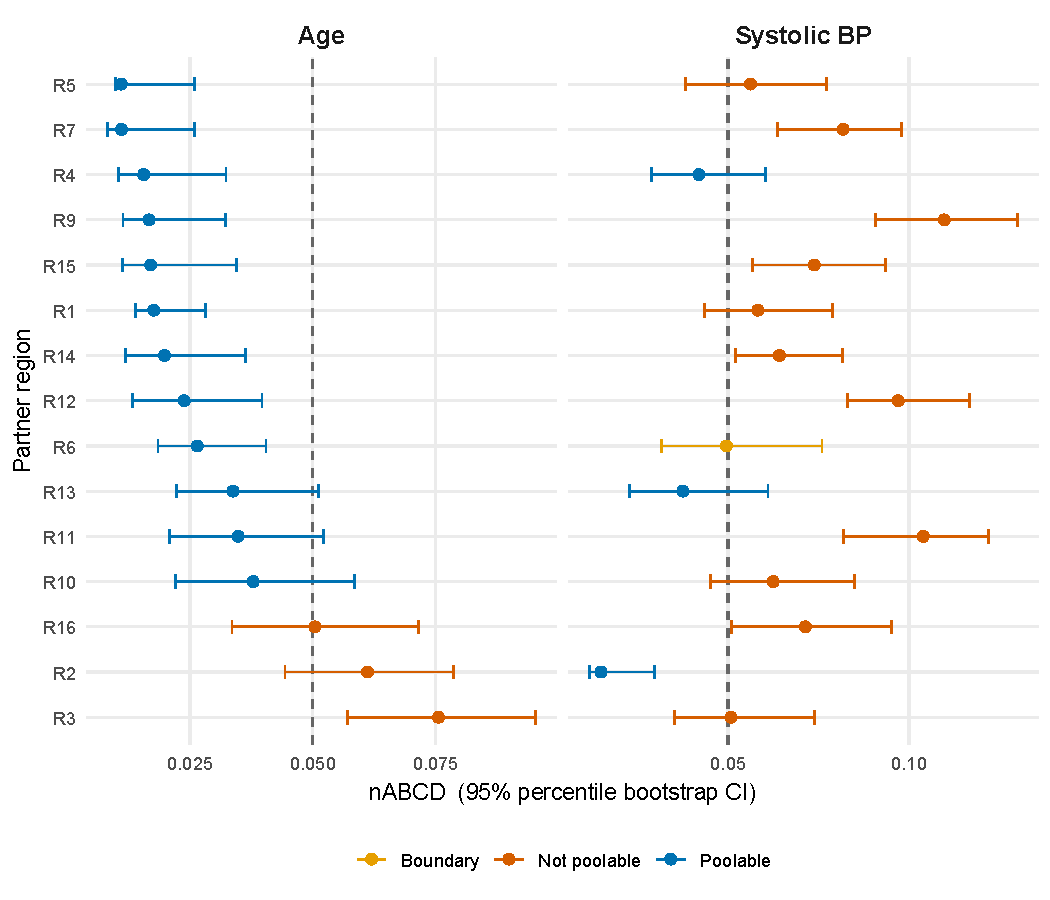
\includegraphics[width=\textwidth]{figures/fig_gusto_r8_forest}
\caption{Forest plot of nABCD with 95\% percentile bootstrap CIs for Region~8 versus each partner region, for age (left) and systolic blood pressure (right). The dashed vertical line indicates the nABCD $= 0.05$ threshold. Blue = poolable; orange = boundary; red = not poolable.}
\label{fig:gusto_forest}
\end{figure}

The two effect modifiers produce strikingly different poolability patterns. For age, 12 of 15 partner regions satisfy the $\text{nABCD} < 0.05$ threshold, with point estimates ranging from 0.011 (R5, R7) to 0.038 (R10). R16 ($\text{nABCD} = 0.050$) falls at the boundary, while R2 (0.061) and R3 (0.076) clearly exceed it. For SBP, only 4 of 15 regions have point estimates below 0.05: R2 (0.015), R13 (0.037), R4 (0.042), and R6 (0.050); the remaining 11 regions range from 0.056 (R5) to 0.110 (R9). The higher SBP nABCD values across most regions reflect greater geographic heterogeneity in blood pressure distributions compared to age.

Two boundary cases merit discussion. R16 has $\text{nABCD}(\text{age}) = 0.050$, placing it at the threshold; its 95\% CI $[0.034, 0.071]$ spans both sides, leaving poolability indeterminate from a statistical standpoint. R6 has $\text{nABCD}(\text{SBP}) = 0.050$, also near the threshold; its 95\% CI $[0.032, 0.076]$ similarly does not resolve the classification. These cases illustrate the value of reporting bootstrap CIs alongside point estimates: the binary poolable/not-poolable determination is supplemented by the uncertainty interval, which informs the degree of confidence in the classification.

An instructive contrast emerges between R2 and R9: R2 has the second-largest age nABCD (0.061) but the smallest SBP nABCD (0.015), while R9 has the second-smallest age nABCD (0.017) but the largest SBP nABCD (0.110). A pooling decision based on either effect modifier alone would reach opposite conclusions for these regions. This underscores the necessity of evaluating all candidate effect modifiers jointly, as visualized in Figure~\ref{fig:gusto_scatter}.

\begin{figure}[ht]
\centering
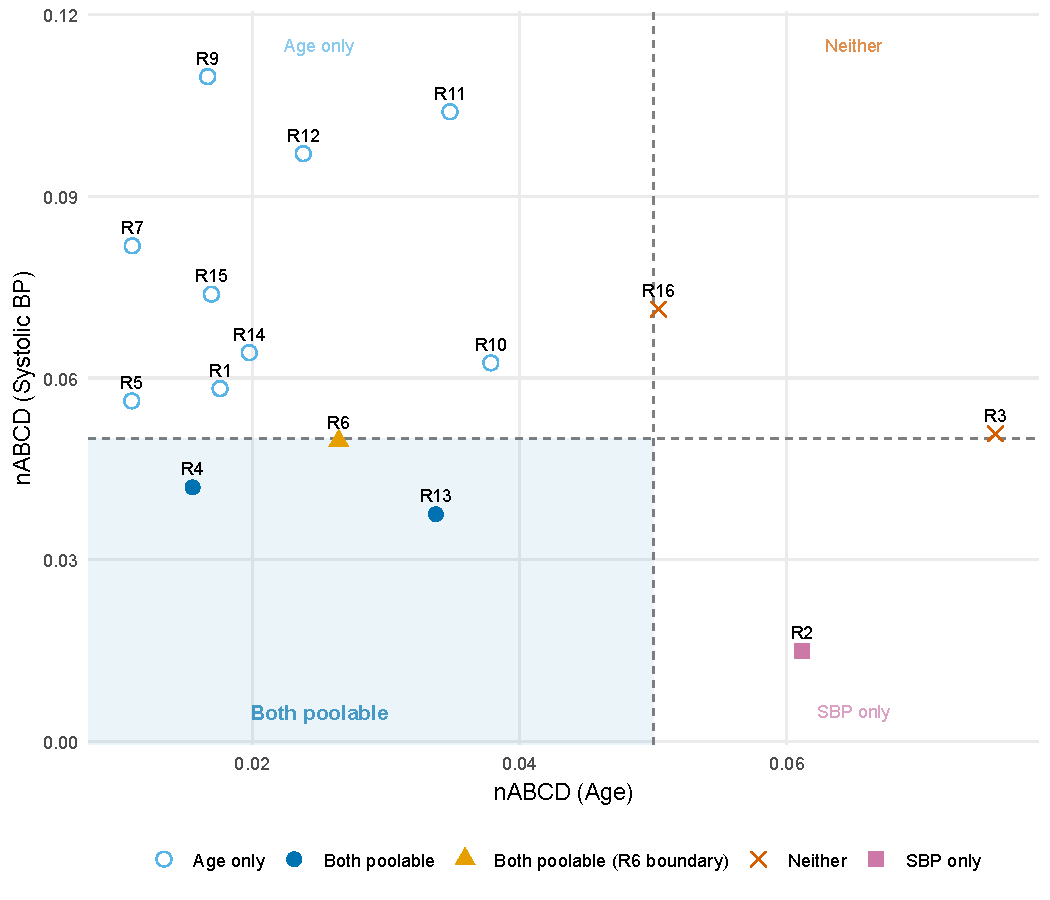
\includegraphics[width=\textwidth]{figures/fig_gusto_r8_scatter}
\caption{Joint pooling assessment for Region~8. Each point represents a partner region, positioned by nABCD for age (horizontal) and SBP (vertical). Dashed lines at nABCD $= 0.05$ create four quadrants. The shaded lower-left quadrant contains regions poolable for both effect modifiers (R4, R6, R13). R2 is poolable for SBP only; many regions are poolable for age only.}
\label{fig:gusto_scatter}
\end{figure}

\subsection{Clinical Calibration: Age}\label{sec:app_age}

Because age is a confirmed effect modifier with estimable CATE sensitivity, clinical calibration translates the observed nABCD values into treatment effect heterogeneity on the clinical outcome scale. Using the FTT-derived estimates ($L_{\text{mean}} = 0.0003$/yr, $L_{\max} = 0.0005$/yr) and equation~(\ref{eq:delta_max}):
\[
\Delta_{\max} = 2L \cdot \text{IQR}_{\text{pooled}} \cdot \text{nABCD}.
\]

Table~\ref{tab:gusto_delta} presents $\Delta_{\max}$ for selected region pairs, using pair-specific $\text{IQR}_{\text{pooled}}$ values (range: 17.0--18.4 years).

\begin{table}[ht]
\caption{Clinical calibration ($\Delta_{\max}$) for age: Region~8 versus selected partners.\label{tab:gusto_delta}}
\begin{tabular*}{\textwidth}{@{\extracolsep\fill}lccccc@{}}
\toprule
\textbf{Partner} & \textbf{nABCD} & \textbf{IQR\textsubscript{pooled}} & \multicolumn{2}{c}{\textbf{$\Delta_{\max}$ (\%pt)}} & \textbf{Pool?} \\
\cmidrule{4-5}
 & & (years) & $L_{\text{mean}}$ & $L_{\max}$ & \\
\midrule
R5  & 0.011 & 17.8 & 0.012 & 0.019 & Y \\
R4  & 0.016 & 17.9 & 0.017 & 0.028 & Y \\
R13 & 0.034 & 17.0 & 0.034 & 0.057 & Y \\
R6  & 0.026 & 17.2 & 0.027 & 0.046 & Y \\
R16 & 0.050 & 17.3 & 0.052 & 0.087 & N$^{\ddagger}$ \\
R2  & 0.061 & 17.6 & 0.064 & 0.107 & N \\
R3  & 0.076 & 17.2 & 0.078 & 0.130 & N \\
\bottomrule
\end{tabular*}
\begin{tablenotes}
\item $\Delta_{\max}$ computed as $2L \times \text{IQR}_{\text{pooled}} \times \text{nABCD}$. FTT-derived estimates: $L_{\text{mean}} = 0.0003$/yr, $L_{\max} = 0.0005$/yr.
\item[$\ddagger$] R16: nABCD at boundary ($= 0.050$).
\end{tablenotes}
\end{table}

For the maximum-nABCD pair (Region~8--R3, $\text{nABCD} = 0.076$):
\begin{itemize}
  \item Using $L_{\max} = 0.0005$/yr: $\Delta_{\max} = 2 \times 0.0005 \times 17.2 \times 0.076 = 0.13$\%pt.
  \item Using $L_{\text{mean}} = 0.0003$/yr: $\Delta_{\max} = 2 \times 0.0003 \times 17.2 \times 0.076 = 0.08$\%pt.
\end{itemize}
These values are negligible relative to the overall treatment effect of thrombolytic therapy in AMI (approximately 2--3\%pt absolute mortality reduction in FTT). Even the non-poolable pair with the largest distributional difference produces a worst-case treatment effect heterogeneity below 0.13\%pt. For the jointly poolable regions, $\Delta_{\max}$ values are smaller still: R13 ($\text{nABCD} = 0.034$) yields $\Delta_{\max} = 0.057$\%pt under $L_{\max}$. Figure~\ref{fig:gusto_calibration}(a) displays the full $\Delta_{\max}$ profile across all 15 partners.

The clinical calibration confirms that age distributional differences across GUSTO-I regions are unlikely to generate clinically meaningful treatment effect heterogeneity for Drug~T, even under conservative assumptions about CATE sensitivity.

\subsection{Sensitivity Analysis: SBP}\label{sec:app_sbp}

Because $L$ for SBP is not estimable from published data, we conduct $L^*$ reverse-calculation analysis (equation~\ref{eq:lstar}) to determine what CATE sensitivity would be required for the observed distributional differences to produce clinically meaningful heterogeneity. Using pair-specific $\text{IQR}_{\text{pooled}}$ values (range: 30--34~mmHg):
\[
L^* = \frac{\Delta_{\text{clin}}}{2 \cdot \text{IQR}_{\text{pooled}} \cdot \text{nABCD}}.
\]

For the maximum-nABCD pair (Region~8--R9, $\text{nABCD} = 0.110$, $\text{IQR}_{\text{pooled}} = 31$~mmHg):
\begin{itemize}
  \item At $\Delta_{\text{clin}} = 1$\%pt: $L^* = 0.01 / (2 \times 31 \times 0.110) = 0.0015$/mmHg.
  \item At $\Delta_{\text{clin}} = 2$\%pt: $L^* = 0.02 / (2 \times 31 \times 0.110) = 0.0029$/mmHg.
\end{itemize}

A CATE sensitivity of $L = 0.0015$/mmHg means that the treatment effect changes by 0.15\%pt for every 1~mmHg change in baseline SBP---a modest value that cannot be ruled out based on published evidence. This suggests that SBP distributional differences between Region~8 and non-poolable partners could plausibly translate into clinically meaningful heterogeneity if a treatment $\times$ SBP interaction exists for Drug~T. Even for pairs closer to the threshold (e.g., R5 with $\text{nABCD} = 0.056$, $\text{IQR}_{\text{pooled}} = 30$~mmHg), $L^* = 0.0030$/mmHg at $\Delta_{\text{clin}} = 1$\%pt---still within a plausible range. Figure~\ref{fig:gusto_calibration}(b) displays the $L^*$ profile across SBP-non-poolable partners.

This sensitivity analysis does not prove that SBP distributional differences will produce treatment effect heterogeneity; rather, it quantifies the conditions under which they would. The modest $L^*$ values indicate that the distributional heterogeneity detected by nABCD warrants explicit consideration in the pooling strategy, even without confirmed effect modifier evidence for SBP.

\begin{figure}[ht]
\centering

\includegraphics[width=\textwidth]{figures/fig_gusto_r8_calibration}
\caption{Clinical interpretation of nABCD values for Region~8. (a)~Age: $\Delta_{\max}$ under two CATE sensitivity assumptions ($L_{\text{mean}} = 0.0003$/yr, $L_{\max} = 0.0005$/yr) for all 15 partner regions, ordered by nABCD. (b)~SBP: $L^*$ (minimum CATE sensitivity to produce $\Delta_{\text{clin}}$) at two clinical thresholds ($\Delta_{\text{clin}} = 1$\%pt, 2\%pt) for the 11 SBP-non-poolable partner regions.}
\label{fig:gusto_calibration}
\end{figure}

\subsection{Pooling Recommendation}\label{sec:app_pooling}

When multiple candidate effect modifiers are evaluated, a region qualifies as a pooling partner only if it satisfies the similarity criterion for every effect modifier---the most restrictive condition governs. Combining the age and SBP assessments:

\begin{itemize}
  \item \textbf{Age}: 12 of 15 regions poolable ($\text{nABCD} < 0.05$); R16 ($\text{nABCD} = 0.050$) falls at the boundary.
  \item \textbf{SBP}: 4 of 15 regions have $\text{nABCD} < 0.05$: R2 (0.015), R13 (0.037), R4 (0.042), and R6 (0.050); R6 is near the boundary ($\text{nABCD} = 0.0496$, 95\% CI $[0.032, 0.076]$).
  \item \textbf{Both effect modifiers}: 3 regions satisfy both criteria---R4, R6, and R13---constituting Region~8's pooling group.
\end{itemize}

R2 is poolable for SBP ($\text{nABCD} = 0.015$) but not for age ($\text{nABCD} = 0.061$); conversely, many regions poolable for age (e.g., R9 with $\text{nABCD}_{\text{age}} = 0.017$) are excluded by SBP ($\text{nABCD}_{\text{SBP}} = 0.110$). This pattern illustrates a central practical implication: the number of eligible pooling partners depends critically on how many effect modifiers are assessed and on the distributional heterogeneity specific to each. In this scenario, SBP---the effect modifier with weaker prior evidence but greater geographic heterogeneity---is the binding constraint.

The R6 boundary case ($\text{nABCD}(\text{SBP}) = 0.0496$) warrants transparent reporting. The point estimate falls marginally below 0.05, but the 95\% CI $[0.032, 0.076]$ encompasses both poolable and non-poolable classifications. Under a strict $< 0.05$ criterion, R6 qualifies; the estimation-centered approach recommends reporting the full CI and $\Delta_{\max}$ (once $L$ becomes available) rather than relying solely on the binary classification. Similarly, R16's $\text{nABCD}(\text{age}) = 0.050$ illustrates that threshold-based decisions at the boundary benefit from the additional information provided by the bootstrap CI and clinical calibration.

The practical consequence for the sponsor is threefold. First, the three confirmed partners (R4, R6, R13) can be designated as Region~8's pooling group for regulatory assessment, with the caveat that R6's SBP classification carries uncertainty. Second, the clinical calibration for age demonstrates that the age-based exclusions (R16, R2, R3) have negligible clinical impact ($\Delta_{\max} < 0.13$\%pt); the substantive pooling constraint arises from SBP distributional differences. Third, if the sponsor obtains additional evidence on SBP---for example, from a Phase~2 interaction analysis or an external database---that evidence can be incorporated through the clinical calibration framework: estimating $L$ for SBP would allow direct $\Delta_{\max}$ computation, potentially expanding or narrowing the pooling set with clinical justification.

Several limitations of this application should be noted:
\begin{enumerate}[1.]
\item \emph{Illustrative data source}: GUSTO-I was not designed as an MRCT; it serves as a convenient publicly available data source for methodological demonstration. In practice, sponsors would assemble regional effect modifier distributions from the most representative and current sources available.
\item \emph{Anonymized regions}: GUSTO-I regions are anonymized, precluding demographic or geographic interpretation of the distributional patterns. This limitation is specific to the dataset, not the framework.
\item \emph{Transferability of $L$}: CATE sensitivity for age was estimated from the FTT meta-analysis of first-generation thrombolytics; the class-transferability assumption to Drug~T requires justification and sensitivity analysis.
\item \emph{Threshold choice}: The $\text{nABCD} < 0.05$ threshold used here is illustrative. In practice, threshold selection should reflect clinical context, regulatory requirements, and the clinical calibration results. The estimation-centered approach (reporting $\Delta_{\max}$ with CIs) provides richer information than a binary poolable/not-poolable determination.
\end{enumerate}
